\begin{figure}[h]
    \centering
    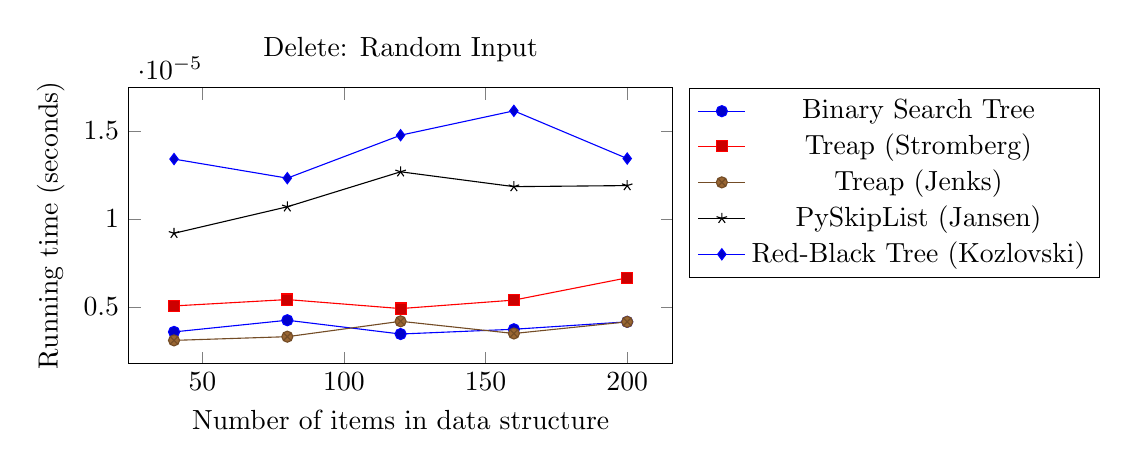
\begin{tikzpicture}
        \begin{axis}[
            xlabel={Number of items in data structure},
            ylabel={Running time (seconds)},
            title={Delete: Random Input},
            width=0.7\textwidth,
            height=2in,
            legend pos=outer north east
        ]
		\addplot coordinates {
			(200, 4.156219647172971e-06)
			(160, 3.73457417572054e-06)
			(120, 3.4635163726440267e-06)
			(80, 4.2465722481985905e-06)
			(40, 3.5839865073449688e-06)
		};
		\addplot coordinates {
			(200, 6.655974942211887e-06)
			(160, 5.391038527854941e-06)
			(120, 4.909157989052212e-06)
			(80, 5.421156061529916e-06)
			(40, 5.05974565742813e-06)
		};
		\addplot coordinates {
			(200, 4.156219647172971e-06)
			(160, 3.493633906319349e-06)
			(120, 4.186337180848293e-06)
			(80, 3.312928704268109e-06)
			(40, 3.1021059685422404e-06)
		};
		\addplot coordinates {
			(200, 1.1896425801691257e-05)
			(160, 1.1836190734340612e-05)
			(120, 1.2679481677245475e-05)
			(80, 1.0691724454683915e-05)
			(40, 9.185847770926125e-06)
		};
		\addplot coordinates {
			(200, 1.343242001912437e-05)
			(160, 1.6142998049890196e-05)
			(120, 1.4757591500832307e-05)
			(80, 1.2318071273143687e-05)
			(40, 1.3402302485449741e-05)
		};
        \legend{Binary Search Tree, Treap (Stromberg), Treap (Jenks), PySkipList (Jansen), Red-Black Tree (Kozlovski)}
        \end{axis}
    \end{tikzpicture}
    \caption{Average of 10 operations, benchmarked every 40, starting at 40.}
\end{figure}